% Drawing 154/06-14 -- folder 154, batch 06, archive page 117 (PDF page 118).
% Transcription: dessin en couleur : une bande horizontale (droites vert clair, ligne médiane brune et verte, tirets jaunes) traversée de droites rouges verticales et de losanges rouges, fermée en haut et en bas par des arcs rouges
% Kind: band crossed by red verticals and lozenges, closed by red arcs. Method 2 (schematic redraw from the facsimile). Status: partial.
% Notes: A horizontal band (light green lines, a brown and green middle line, yellow dashes) crossed by red vertical lines and red lozenges, closed at the top and the bottom by red arcs; light green verticals at the ends. Read from the page view; the count of verticals and lozenges is approximate (about seven verticals, three lozenges). Still differs from the facsimile: Read from the page view; the count of verticals and lozenges is approximate (about seven verticals, three lozenges).
% Coordinates: 1 unit = 1 mm = 1/100 of the crop width (bbox in page fractions: [0.148, 0.377, 0.365, 0.46]).
% Redrawn by Claude (claude-opus-5-5), issue #73, 2026-11-07; not checked by a human; not compiled (no TeX in the session).
% Revised by Claude (claude-opus-5-5) 2026-11-09 (issue #128) after Michel's check: vertices snapped to exact intersections (drawn points on their lines, meeting ends on the stroke they meet, near-concurrent lines through one computed point, curve ends on their rim); labels at \small as in folder 80 batch 3. Status: partial.
% Rights: reproduces part of the work -- behind RENDER_TRANSCRIPTS, never published by itself.
\documentclass[tikz,border=3pt]{standalone}
\usepackage{amsmath,amssymb}
\usetikzlibrary{patterns,arrows.meta}
\tikzset{Or/.style={orange!90!black}, Ye/.style={yellow!80!orange}, Lg/.style={green!60!black!70}, Dg/.style={green!45!black}, Br/.style={brown!80!black}, Rd/.style={red!85!black}, Bl/.style={blue!70!black}, Gy/.style={black!40}, pencil/.style={black!45}, struck/.style={black!35}, mark/.style={circle,draw,inner sep=1.3pt}, pt/.style={circle,fill,inner sep=0.9pt}, opt/.style={circle,draw,fill=white,inner sep=1.1pt}}
\begin{document}
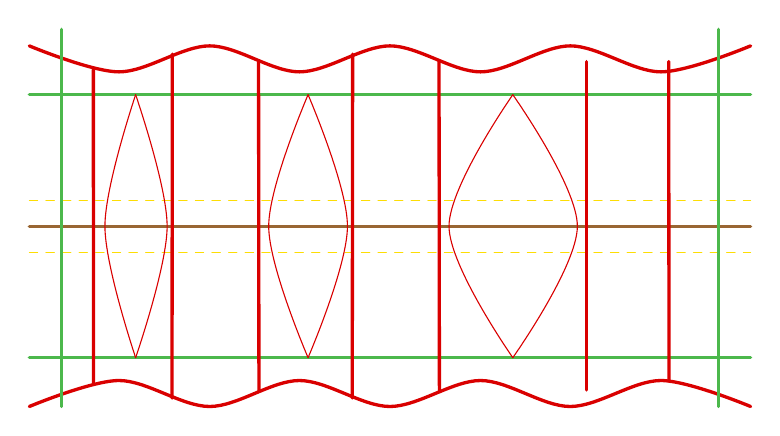
\begin{tikzpicture}[x=1mm,y=1mm,line cap=round,line join=round,font=\scriptsize]
\draw[Lg,very thick] (4.2,-10.4) -- (95.8,-10.4);
\draw[Lg,very thick] (4.2,-43.8) -- (95.8,-43.8);
\draw[Br,very thick] (4.2,-27.1) -- (95.8,-27.1);
\draw[Ye,dashed] (4.2,-23.8) -- (95.8,-23.8);
\draw[Ye,dashed] (4.2,-30.4) -- (95.8,-30.4);
\draw[Rd,very thick] plot[smooth, tension=0.55] coordinates {(4.2,-4.2) (15.6,-7.5) (27.1,-4.2) (38.5,-7.5) (50,-4.2) (61.5,-7.5) (72.9,-4.2) (84.4,-7.5) (95.8,-4.2)};
\draw[Rd,very thick] plot[smooth, tension=0.55] coordinates {(4.2,-50) (15.6,-46.7) (27.1,-50) (38.5,-46.7) (50,-50) (61.5,-46.7) (72.9,-50) (84.4,-46.7) (95.8,-50)};
\draw[Rd,very thick] (12.33,-7.21) -- (12.35,-46.99);
\draw[Rd,very thick] (22.36,-5.25) -- (22.32,-48.93);
\draw[Rd,very thick] (33.31,-6.18) -- (33.36,-48);
\draw[Rd,very thick] (45.26,-5.24) -- (45.21,-48.93);
\draw[Rd,very thick] (56.23,-6.15) -- (56.28,-48.03);
\draw[Rd,very thick] (75,-6.2) -- (75,-47.9);
\draw[Rd,very thick] (85.4,-6.2) -- (85.44,-46.74);
\draw[Rd] plot[smooth, tension=0.55] coordinates {(17.7,-10.4) (13.8,-27.1) (17.7,-43.8)};
\draw[Rd] plot[smooth, tension=0.55] coordinates {(17.7,-10.4) (21.7,-27.1) (17.7,-43.8)};
\draw[Rd] plot[smooth, tension=0.55] coordinates {(39.6,-10.4) (34.6,-27.1) (39.6,-43.8)};
\draw[Rd] plot[smooth, tension=0.55] coordinates {(39.6,-10.4) (44.6,-27.1) (39.6,-43.8)};
\draw[Rd] plot[smooth, tension=0.55] coordinates {(65.6,-10.4) (57.5,-27.1) (65.6,-43.8)};
\draw[Rd] plot[smooth, tension=0.55] coordinates {(65.6,-10.4) (73.8,-27.1) (65.6,-43.8)};
\draw[Lg,very thick] (8.3,-2.1) -- (8.3,-50);
\draw[Lg,very thick] (91.7,-2.1) -- (91.7,-50);
\end{tikzpicture}
\end{document}
